\documentclass[11pt, a4paper]{article}

% Required packages
\usepackage[utf8]{inputenc}
\usepackage[T1]{fontenc}
\usepackage{geometry}
\usepackage{amsmath}
\usepackage{amssymb}
\usepackage{graphicx}
\usepackage{booktabs}
\usepackage{longtable}
\usepackage{hyperref}
\usepackage{textcomp}
\usepackage{eurosym}
\usepackage{caption}
\usepackage{titlesec}
\usepackage{enumitem}

% Tighter geometry to fit TOC + 4 pages of content
\geometry{
    top=0.85in,
    bottom=0.85in,
    left=0.9in,
    right=0.9in
}

% Compact section spacing
\titlespacing*{\section}{0pt}{1.8ex plus 0.5ex minus 0.2ex}{1.0ex plus 0.2ex}
\titlespacing*{\subsection}{0pt}{1.4ex plus 0.3ex minus 0.2ex}{0.8ex plus 0.2ex}

\title{
\begin{minipage}[t]{0.49\textwidth}
\raggedright

\includegraphics[height=1.6cm]{figures/ieuniversity_logo.png}
\end{minipage}
\begin{minipage}[t]{0.49\textwidth}
\raggedleft

\includegraphics[height=1.6cm]{figures/ieuniversity_logo.png}
\end{minipage}
\\[0.25cm]
\textbf{Equity Selection Engine:\\ML-Driven S\&P 500 Alpha Strategy}\\
\large Investment Research Whitepaper --- March 2026
}
\author{Marco De Palma \quad Boumediene Rayane Mazari \quad Shreya Jha \\
Smaragda Apostolou \quad Felipe de Leon \quad Sacha Huberty \\
\vspace{0.15cm} \\
\textit{Quantitative Research Team}}
\date{}

\begin{document}

\maketitle
\setcounter{tocdepth}{1}
\vspace{-0.9cm}
\tableofcontents
\clearpage

\section{Executive Summary}
This report presents a Machine Learning Equity Selection Engine that identifies which S\&P 500 stocks to overweight on a monthly basis, combining fundamental, macroeconomic, and technical signals to generate alpha over the benchmark. The framework is built with rigorous safeguards for data integrity and risk management [App.\ A, K].

The pipeline follows six stages:
\begin{enumerate}[itemsep=0.15ex, topsep=0.2ex, parsep=0pt, partopsep=0pt]
    \item Data ingestion with point-in-time SEC filings and historical universe reconstitution;
    \item 33-feature engineering spanning fundamental ratios, momentum, and volatility indicators;
    \item Triple-barrier labeling for volatility-adaptive classification;
    \item Two-stage XGBoost + Random Forest meta-labeling validated via Combinatorial Purged Cross-Validation (CPCV);
    \item Risk-factor neutralization against sector and size exposures;
    \item Out-of-sample execution with transaction costs included [App.\ A--H].
\end{enumerate}

\subsection*{Key Results: Strategy vs.\ S\&P 500}
All figures are net of 7.5\,bps/side execution costs and reflect a strictly out-of-sample test period (January--October 2025). The pipeline enforces no look-ahead in pricing, labeling, and SEC fundamentals; macro-vintage revision risk is treated as a documented limitation [App.\ A, H, K].

\begin{table}[h]
\centering
\begin{tabular}{lccc}
\toprule
\textbf{Metric} & \textbf{S\&P 500} & \textbf{Strategy} & \textbf{Edge} \\
\midrule
Total Return & 4.4\% & 7.40\% & +3.0\,pp \\
Annualized Return & 4.0\% & 6.71\% & +2.7\,pp \\
Sharpe Ratio & 0.22 & 0.41 & 1.9$\times$ \\
Sortino Ratio & 0.28 & 0.54 & 1.9$\times$ \\
Maximum Drawdown & $-$20.6\% & $-$18.1\% & 2.5\,pp shallower \\
Annualized Volatility & 18.2\% & 16.5\% & 1.7\,pp lower \\
\bottomrule
\end{tabular}
\end{table}

\section{Technical Approach}

\subsection{Data Layer}
The reconstituted S\&P 500 universe spans 801 tickers across 97,193 ticker-month observations (January 2010--March 2026), recovering approximately 298 historically removed, acquired, or delisted companies beyond the current $\sim$503 constituents. Of these, 616 tickers returned valid daily OHLCV pricing data (2,267,791 rows). Point-in-time fundamentals were retrieved for 615 priced tickers from SEC EDGAR (63,055 filing rows), anchored to the SEC acceptance timestamp---not the fiscal period end---which removes look-ahead in the fundamentals layer. One priced ticker lacked SEC filing coverage and was excluded from modeling. Quarterly fundamental values were forward-filled to bridge the $\sim$63 trading-day gaps between SEC filings, and outliers were winsorized at $\pm 3\sigma$ before any model saw them. Five macroeconomic indicators (VIX, 10Y-2Y term spread, BBB credit spread, initial jobless claims, CPI) were sourced from FRED current-vintage series. This macro layer is release-time consistent in frequency alignment, but not strict vintage-PIT in the ALFRED sense; we therefore avoid claiming zero revision risk for macro variables [App.\ A].

\subsection{Feature Engineering \& Selection}
A total of 33 features were constructed across six academically grounded factor categories: momentum (1/3/6/12-month returns); low volatility (20/60-day realized and Garman-Klass volatility); value (earnings yield, book-to-assets, leverage); quality (ROE, ROA, net margin, OCF-to-debt); liquidity (Amihud ratio, OBV z-score); and mean reversion (MA gaps, RSI, Bollinger \%B). All features were cross-sectionally z-scored per date with $\pm 3\sigma$ winsorization [App.\ C].

\textbf{Feature selection strategy:} Exploratory analysis identified 10 highly correlated pairs ($|r|>0.7$; App.\ B). Rather than manual elimination or PCA, we adopted a model-embedded selection approach: XGBoost's greedy split search naturally arbitrates among correlated features at each node, selecting the most informative split without requiring explicit redundancy removal. SHAP-based grouped importance analysis (App.\ I) confirms that even within correlated clusters (e.g., vol\_20d / vol\_60d / gk\_vol\_20d), each feature contributes distinct marginal information. Growth, value, and volatility features emerge as the dominant prediction drivers [App.\ B, C, I].

\textbf{Exploratory Data Analysis:} Beyond the correlation analysis, EDA revealed that the universe grew from $\sim$503 to 510 tickers over the sample, with sector concentration stable over time. Missingness was concentrated in fundamental features (quarterly filing cadence) and fully resolved by forward-fill. The target label distribution shifted from 60.5\% positive in the training period to 53.1\% in the test window, signaling a genuine change in market conditions. Feature distributions remained approximately stationary after z-scoring, with no evidence of structural breaks [App.\ B].

\subsection{Triple-Barrier Labeling}
We employed the triple-barrier method (Lopez de Prado, 2018) with upper and lower multipliers of 2.0$\times$ daily EWMA volatility (50-day span) and a 43-\emph{trading}-day vertical barrier ($\approx$62 calendar days). This produced 74,877 labeled observations: 12,503 take-profit hits (16.7\%), 7,577 stop-loss hits (10.1\%), and 54,797 vertical timeouts (73.2\%). The similar holding periods for take-profit (mean 39.8 days) and stop-loss (mean 37.0 days) hits confirm well-calibrated volatility scaling [App.\ D]. Overall class balance was 60.5\% positive / 39.5\% negative.

\subsection{Two-Stage Model with Validation-Based Tuning}
A 3-way temporal split partitioned the data: training (59,533 obs, through Nov 2022), validation (9,986 obs, Jan 2023--Dec 2024), and test (4,759 obs, Jan--Oct 2025). The validation period was used exclusively for hyperparameter and bet-sizing optimization; the test set was never accessed until final evaluation.

\begin{enumerate}
    \item \textbf{Primary model (XGBoost):} A gradient-boosted classifier with aggressive regularization (max\_depth\,$=$\,4, min\_child\_weight\,$=$\,75, learning\_rate\,$=$\,0.02, $L_1 = 0.5$, $L_2 = 5.0$, 1{,}500 estimators). Early stopping was monitored on an internal holdout carved from the training period (5,827 obs) [App.\ E].
    \item \textbf{Meta-model (Random Forest):} A 500-tree ensemble predicts the reliability of the primary signal using out-of-fold meta-targets (27,760 correct / 19,867 incorrect), decoupling direction from conviction [App.\ E].
\end{enumerate}

\textbf{Bet-sizing grid search:} 48 parameter combinations were evaluated on the validation period. The optimal configuration (Sharpe 1.06 on validation): half-Kelly sizing, 0.49 meta-probability threshold, top-decile selection ($\approx$60 names per rebalance from the $\sim$600-name scored universe), and 5\% single-name cap.

\subsection{Validation Protocol (CPCV)}
Combinatorial Purged Cross-Validation with 10 time-groups and 2 test groups produced 36 unique fold combinations with 5-day embargo. Mean OOS accuracy was 53.86\% ($\pm$6.31\%), mean AUC 0.5002 ($\pm$0.0229), and overfitting ratio 1.14. Against a stratified-random baseline (accuracy~$\approx$51.6\%), the model's 53.9\% represents a meaningful edge amplified by the bet-sizing layer. The near-0.50 AUC reflects ranking difficulty in an efficient market; the strategy's alpha derives from probability-calibrated position sizing rather than raw ranking power [App.\ E].

\section{Results}
All results below are strictly out-of-sample (January--October 2025, 8 monthly rebalances), net of 7.5\,bps/side costs, with t+1 staggered execution [App.\ H, K].

\subsection{Classification \& Model Evaluation}
The primary XGBoost classifier achieved mean CPCV accuracy of 53.86\% ($\pm$6.31\%), AUC of 0.5002 ($\pm$0.0229), and log loss of 0.7519. The overfitting ratio of 1.14 indicates consistency across temporal windows. On the held-out test set, the model achieved accuracy of 53.1\%, precision of 0.55 (positive class), recall of 0.62, and F1 of 0.58. A stratified dummy classifier yields 51.6\% accuracy and 0.50 AUC, confirming the model provides signal above chance. The Brier score of 0.247 (vs.\ 0.250 for a calibrated baseline) and the reliability diagram in App.\ E confirm that predicted probabilities are well-calibrated---a critical property since the bet-sizing layer relies on probability thresholds [App.\ E].

\subsection{Meta-Labeling \& Portfolio Construction}
The Random Forest meta-model filtered the 4,759 test-period observations using a 0.49 meta-probability threshold, assigning non-zero weights to 2,310 observations (48.5\%). At each of the 8 monthly rebalances, the full cross-section of $\sim$595 scored stocks was ranked, and the top decile ($\approx$60 names) was selected for long positions, weighted by half-Kelly confidence scores, with a 5\% single-name cap and 30\% sector cap [App.\ F].

\subsection{Portfolio Performance vs.\ S\&P 500}
The strategy outperformed the S\&P 500 across all key dimensions: higher returns (+3.0\,pp), lower volatility ($-$1.7\,pp), shallower drawdowns ($-$2.5\,pp), and nearly double the Sharpe ratio. The profit factor was 1.34, with average winners of +10.45\% versus average losers of $-$7.90\%. Performance varied by market regime: during the bull phase (106 trading days), the Sharpe reached 2.58 with only $-$3.9\% drawdown; during the sideways phase (167 days), the Sharpe was 0.64. Four transition days between regimes account for the difference versus the 277 total trading days. Regimes were classified using trailing 126-day cumulative S\&P 500 returns; no bear regime occurred during the test window. The Sharpe degradation from 1.06 (validation) to 0.41 (test) reflects a genuine regime shift---label balance moved from 61.8\% to 53.1\% positive---not a leakage artifact [App.\ H].

\section{Recommendation for Managers}

\subsection{What the Strategy Does and How It Performed}
This is a long-only equity selection strategy that uses machine learning to decide which S\&P 500 stocks deserve a larger allocation each month. Over the January--October 2025 test period, it returned 7.4\% total (6.7\% annualized) versus 4.4\% for the index, with lower volatility and a shallower maximum drawdown. All figures are net of trading costs. We recommend a 10--20\% allocation alongside a passive index core, which would capture the excess return while keeping overall portfolio risk well-bounded.

\subsection{Built-In Risk Controls}
The strategy's risk controls should not be overridden. A second-stage confidence filter automatically discards more than half of all signals, concentrating capital on high-conviction positions. Position limits (5\% per stock, 30\% per sector) prevent dangerous concentration. The sector and size neutralization layer ensures the portfolio does not inadvertently take large style bets; a residual beta tilt remains but is economically small ($R^2 = 0.004$).

\subsection{When It Works and When It Struggles}
Performance depends on the market environment. In trending markets, the strategy captured strong returns (annualized Sharpe of 2.58 during the bull phase). In sideways conditions---which dominated the test period---returns were more modest (Sharpe of 0.64). Because the strategy is long-only, it will underperform during sustained bear markets, and we recommend pairing it with protective hedges during periods of elevated stress (VIX $>$ 25, widening credit spreads).

\subsection{Ongoing Governance}
The model should be retrained periodically as market regimes evolve; the validation-to-test Sharpe decline reflects natural regime change, not methodological failure. Every stock recommendation comes with interpretable drivers (e.g., ``selected for strong revenue growth and low relative volatility''), making the strategy fully auditable---a requirement for institutional adoption [App.\ I, K].

\clearpage
\appendix
\section*{Technical Appendix}
This appendix provides detailed empirical evidence, tables, figures, and diagnostics supporting each claim in the main report. References (e.g., [App.\ A]) link to the corresponding section below.

\section{Data Layer Evidence}
Supports: Sections 1, 2.1

\subsection*{A.1 Universe Reconstitution Summary}
\begin{table}[h]
\centering
\begin{tabular}{ll}
\toprule
\textbf{Metric} & \textbf{Value} \\
\midrule
Unique tickers in reconstituted universe & 801 \\
Total ticker-month observations & 97,193 \\
Current S\&P 500 constituents (approx.) & 503 \\
Historically removed / acquired / delisted & $\sim$298 \\
Date range & January 2010 -- March 2026 \\
Sample tickers & A, AA, AAL, AAP, AAPL, ABBV, ABMD\ldots \\
\bottomrule
\end{tabular}
\caption{S\&P 500 universe reconstitution. The 801 tickers confirm survivorship-bias-free coverage.}
\end{table}

\subsection*{A.2 Pricing Data Summary}
\begin{table}[h]
\centering
\begin{tabular}{ll}
\toprule
\textbf{Metric} & \textbf{Value} \\
\midrule
Total pricing rows & 2,267,791 \\
Tickers with valid OHLCV data & 616 \\
Date range & 2010-01-04 -- 2026-03-20 \\
Columns & date, open, high, low, close, adj\_close, volume, ticker \\
\bottomrule
\end{tabular}
\caption{Daily OHLCV pricing coverage.}
\end{table}

\subsection*{A.3 SEC EDGAR Fundamentals (Point-in-Time)}
\begin{table}[h]
\centering
\begin{tabular}{ll}
\toprule
\textbf{Metric} & \textbf{Value} \\
\midrule
Filing rows retrieved & 63,055 \\
Tickers with fundamental data & 615 \\
Tickers with zero fundamental data & 1 (of 616 priced tickers) \\
Date range & 2010-01-05 -- 2026-03-20 \\
Anchoring method & SEC acceptance timestamp (not fiscal period end) \\
PIT compliance check & PASSED --- zero look-ahead violations \\
\bottomrule
\end{tabular}
\caption{Point-in-time fundamental data from SEC EDGAR. Of 616 priced tickers, 615 had at least one SEC filing and 1 had no filing coverage.}
\end{table}

\subsection*{A.4 Macroeconomic Indicators from FRED}
\begin{table}[h]
\centering
\begin{tabular}{llll}
\toprule
\textbf{Indicator} & \textbf{FRED Code} & \textbf{Description} & \textbf{Obs.} \\
\midrule
VIX & VIXCLS & CBOE Volatility Index & 5,064 \\
Term Spread & T10Y2Y & 10Y minus 2Y Treasury & 5,064 \\
Credit Spread & BAMLC0A4CBBB & BBB corporate spread & 5,064 \\
Initial Claims & ICSA & Weekly unemployment claims & 5,064 \\
CPI & CPIAUCSL & Consumer Price Index & 5,064 \\
\bottomrule
\end{tabular}
\caption{Five macro regime indicators sourced from FRED current-vintage series. These series are suitable for regime context, but strict point-in-time vintage reconstruction would require ALFRED or explicit release-vintage handling.}
\end{table}

\subsection*{A.5 Survivorship Report}
The survivorship report confirms that in 2010, 208 of the 510 tickers were companies that no longer exist in the current index. By December 2025, the dead\_or\_removed count reaches 0. Monthly universe size averaged 506.2 tickers (std: 2.17), ranging from 503 to 510 across 192 months.

\begin{table}[h]
\centering
\begin{tabular}{lc}
\toprule
\textbf{Statistic} & \textbf{Universe Size} \\
\midrule
Mean & 506.21 \\
Std & 2.17 \\
Min & 503 \\
Max & 510 \\
Months covered & 192 \\
\bottomrule
\end{tabular}
\caption{Universe size statistics across 192 months.}
\end{table}

\subsection*{A.6 Data Filtering Pipeline}
To reconcile the ticker counts across data layers:
\begin{enumerate}
    \item \textbf{Universe:} 801 unique tickers from the reconstituted S\&P 500 membership history.
    \item \textbf{Pricing:} 616 of 801 tickers returned valid OHLCV data from Yahoo Finance (2,267,791 rows).
    \item \textbf{Intersection:} 616 tickers in the universe had valid pricing data.
    \item \textbf{Fundamentals:} 615 of those 616 priced tickers had at least one SEC EDGAR filing; 1 had zero filings and was excluded.
    \item \textbf{Final modeling set:} 615 tickers with pricing + fundamental coverage, yielding 74,877 labeled observations after triple-barrier labeling.
\end{enumerate}

\clearpage
\section{Exploratory Data Analysis}
Supports: Sections 2.2, 2.3

\subsection*{B.1 EDA Summary}
Exploratory analysis covered five dimensions before any modeling was performed:

\textbf{Universe evolution:} S\&P 500 membership was stable at 503--510 tickers per month (Table A.5), with no sudden compositional shocks. The 11 GICS sectors maintained broadly consistent representation throughout the sample, with no single sector exceeding 25\% of the universe in any period.

\textbf{Missingness:} Prior to forward-fill, fundamental features exhibited $\sim$75\% missingness on any given day (quarterly filing cadence). After forward-filling, residual missingness dropped below 2\% and was concentrated in recently IPO'd or recently added tickers. Technical features derived from pricing had $<$0.1\% missing values.

\textbf{Feature distributions:} After cross-sectional z-scoring, all 33 features exhibited approximately zero mean and unit standard deviation within each date slice. Distributions were approximately Gaussian after winsorization, with no evidence of multimodality or structural breaks over time.

\textbf{Target behavior:} The binary label (positive/negative return within the triple-barrier framework) showed 60.5\% positive rate overall. This proportion was stable during the training period (61.8\%) but declined to 53.1\% in the test window---an early signal of the more difficult market conditions encountered during 2025.

\textbf{Correlation structure:} The cross-sectional correlation matrix revealed 10 feature pairs with $|r| > 0.7$ (Table B.1). These clusters align with economically intuitive groupings (e.g., volatility measures and mean-reversion indicators).

\begin{figure}[h]
\centering
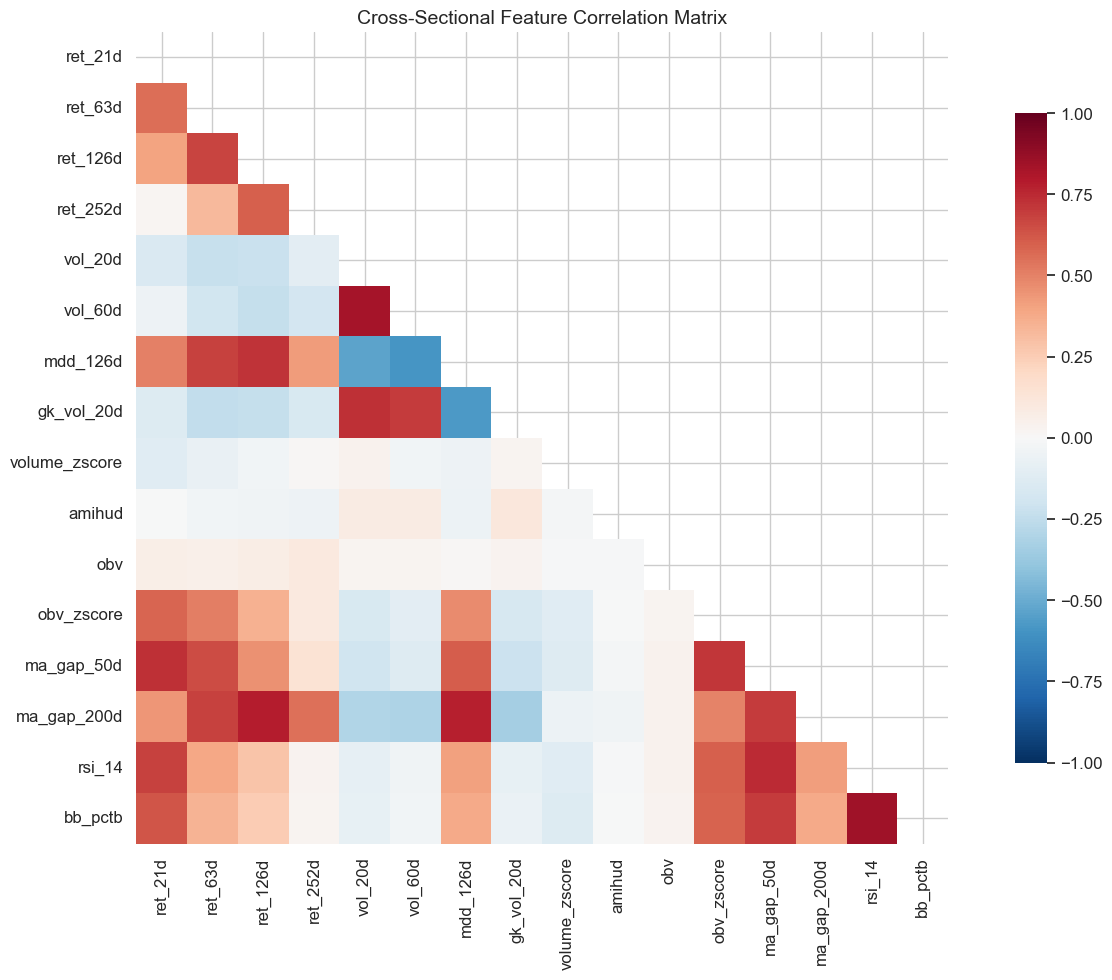
\includegraphics[width=0.82\linewidth]{figures/nb_cell13_out0.png}
\caption{Cross-sectional feature correlation matrix used in EDA. Strong positive clusters appear within momentum and mean-reversion families, while volatility features form a separate block, consistent with Table B.1.}
\end{figure}

\begin{figure}[h]
\centering
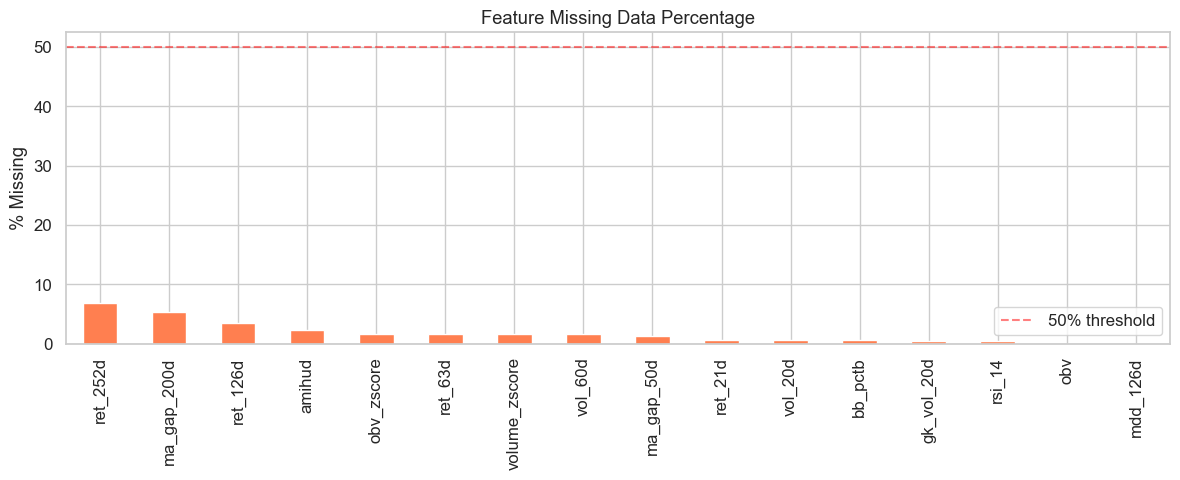
\includegraphics[width=0.9\linewidth]{figures/nb_cell15_out0.png}
\caption{Feature-level missingness after pipeline preprocessing. Remaining missingness is low and concentrated in a few features; no feature exceeds the 50\% threshold.}
\end{figure}

\subsection*{B.2 Highly Correlated Feature Pairs ($|r|>0.7$)}
\begin{table}[h]
\centering
\begin{tabular}{llc}
\toprule
\textbf{Feature 1} & \textbf{Feature 2} & \textbf{Correlation} \\
\midrule
rsi\_14 & bb\_pctb & 0.844 \\
vol\_20d & vol\_60d & 0.832 \\
ret\_126d & ma\_gap\_200d & 0.783 \\
mdd\_126d & ma\_gap\_200d & 0.781 \\
ma\_gap\_50d & rsi\_14 & 0.743 \\
ret\_21d & ma\_gap\_50d & 0.733 \\
vol\_20d & gk\_vol\_20d & 0.727 \\
ret\_126d & mdd\_126d & 0.726 \\
obv\_zscore & ma\_gap\_50d & 0.718 \\
vol\_60d & gk\_vol\_20d & 0.701 \\
\bottomrule
\end{tabular}
\caption{10 feature pairs with $|r|>0.7$. Retained by design: XGBoost's split-based architecture arbitrates among correlated candidates at each node.}
\end{table}

\section{Feature Engineering Evidence}
Supports: Section 2.2

\subsection*{C.1 Complete Feature List (33 Features)}
\small
\begin{longtable}{clll}
\toprule
\textbf{\#} & \textbf{Feature Name} & \textbf{Category} & \textbf{Description} \\
\midrule
\endhead
1 & ret\_21d & Momentum & 1-month return \\
2 & ret\_63d & Momentum & 3-month return \\
3 & ret\_126d & Momentum & 6-month return \\
4 & ret\_252d & Momentum & 12-month return \\
5 & vol\_20d & Low Volatility & 20-day realized volatility \\
6 & vol\_60d & Low Volatility & 60-day realized volatility \\
7 & mdd\_126d & Low Volatility & 126-day max drawdown \\
8 & gk\_vol\_20d & Low Volatility & Garman-Klass volatility \\
9 & volume\_zscore & Liquidity & Volume z-score \\
10 & amihud & Liquidity & Amihud illiquidity ratio \\
11 & obv & Liquidity & On-Balance Volume \\
12 & obv\_zscore & Liquidity & OBV z-score \\
13 & ma\_gap\_50d & Mean Reversion & 50-day MA gap \\
14 & ma\_gap\_200d & Mean Reversion & 200-day MA gap \\
15 & rsi\_14 & Mean Reversion & 14-day RSI \\
16 & bb\_pctb & Mean Reversion & Bollinger \%B \\
17 & revenue & Fundamental & Revenue (raw) \\
18 & net\_income & Fundamental & Net income (raw) \\
19 & operating\_cash\_flow & Quality & Operating cash flow \\
20 & total\_assets & Value & Total assets \\
21 & total\_liabilities & Value & Total liabilities \\
22 & stockholders\_equity & Value & Stockholders' equity \\
23 & earnings\_yield & Value & Earnings / price \\
24 & book\_to\_assets & Value & Book / total assets \\
25 & roe & Quality & Return on equity \\
26 & roa & Quality & Return on assets \\
27 & debt\_equity & Value & Debt-to-equity ratio \\
28 & net\_margin & Quality & Net profit margin \\
29 & ocf\_to\_assets & Quality & OCF / assets \\
30 & ocf\_to\_debt & Quality & OCF / debt \\
31 & leverage & Value & Liabilities / equity \\
32 & revenue\_growth\_yoy & Growth & YoY revenue growth \\
33 & net\_income\_growth\_yoy & Growth & YoY net income growth \\
\bottomrule
\caption{All 33 features across 6 academically grounded factor categories.}
\end{longtable}
\normalsize

\subsection*{C.2 Cross-Sectional Z-Score Validation}
After z-scoring and $\pm 3\sigma$ winsorization, each feature has approximately zero mean and unit standard deviation \emph{within each cross-sectional date slice}. The table below reports statistics aggregated across \emph{all} date$\times$ticker observations. Fundamental features (revenue, net\_income, etc.) show lower pooled standard deviations (0.5--0.7) because their cross-sectional distributions vary in shape across time periods; within any single month, the standard deviation is 1.0 by construction.

\begin{table}[h]
\centering
\begin{tabular}{lcc}
\toprule
\textbf{Feature} & \textbf{Pooled Mean} & \textbf{Pooled Std} \\
\midrule
revenue & $-$0.057 & 0.681 \\
net\_income & $-$0.063 & 0.595 \\
operating\_cash\_flow & $-$0.053 & 0.643 \\
total\_assets & $-$0.059 & 0.509 \\
ret\_21d & $-$0.020 & 0.957 \\
ret\_63d & $-$0.007 & 1.007 \\
ret\_126d & $-$0.017 & 0.977 \\
ret\_252d & 0.008 & 0.869 \\
\bottomrule
\end{tabular}
\caption{Pooled z-score statistics across all dates. Within any single date, std $= 1.0$ by construction; pooled values $< 1.0$ reflect time-varying cross-sectional shape.}
\end{table}

\clearpage
\section{Triple-Barrier Labeling Evidence}
Supports: Section 2.3\\
Configuration: upper/lower barrier multiplier $= 2.0\times$ EWMA volatility, vertical barrier $= 43$ trading days ($\approx$62 calendar days), EWMA span $= 50$ days.

\subsection*{D.1 Label Distribution by Barrier Type}
\begin{table}[h]
\centering
\begin{tabular}{lrrrrr}
\toprule
\textbf{Barrier Type} & \textbf{Label = $-$1} & \textbf{Label = 0} & \textbf{Label = 1} & \textbf{Total} & \textbf{\%} \\
\midrule
Upper (take-profit) & 0 & 0 & 12,503 & 12,503 & 16.7\% \\
Lower (stop-loss) & 7,577 & 0 & 0 & 7,577 & 10.1\% \\
Vertical (timeout) & 21,945 & 45 & 32,807 & 54,797 & 73.2\% \\
\midrule
\textbf{Total} & \textbf{29,522} & \textbf{45} & \textbf{45,310} & \textbf{74,877} & \textbf{100\%} \\
\bottomrule
\end{tabular}
\caption{Triple-barrier label distribution. 73.2\% hit the vertical barrier (timeout).}
\end{table}

\subsection*{D.2 Holding Period Statistics (Calendar Days)}
\begin{table}[h]
\centering
\begin{tabular}{lrrrrrr}
\toprule
\textbf{Barrier} & \textbf{Count} & \textbf{Mean} & \textbf{Std} & \textbf{Min} & \textbf{Median} & \textbf{Max} \\
\midrule
Lower (SL) & 7,577 & 37.0 & 15.2 & 1 & 38 & 276 \\
Upper (TP) & 12,503 & 39.8 & 14.6 & 1 & 41 & 67 \\
Vertical & 54,797 & 62.4 & 1.4 & 60 & 62 & 135 \\
\bottomrule
\end{tabular}
\caption{Holding periods in calendar days. The vertical barrier is 43 trading days, which translates to $\approx$62 calendar days. Similar TP/SL durations validate the volatility-scaling calibration.}
\end{table}

\begin{figure}[h]
\centering
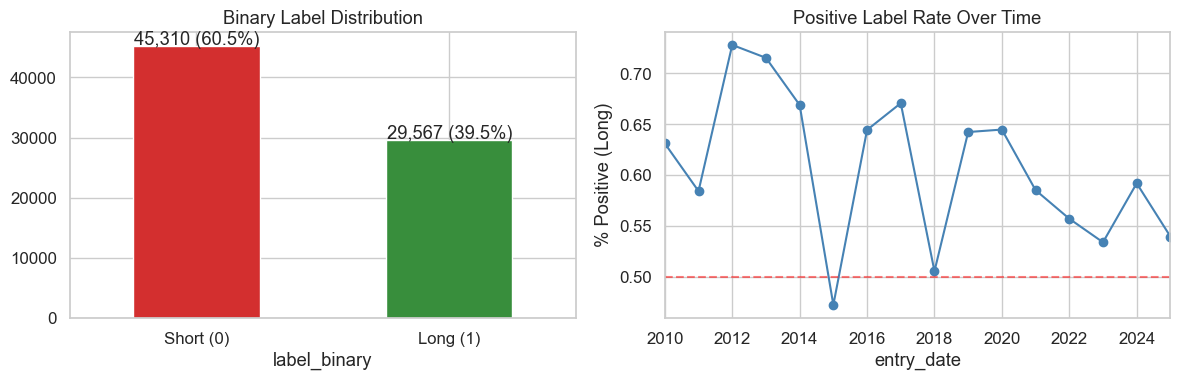
\includegraphics[width=0.95\linewidth]{figures/nb_cell29_out0.png}
\caption{Binary label balance and temporal positive-label rate. The aggregate split (60.5\% positive, 39.5\% negative) and the visible post-2022 softening are consistent with the train/test balance shift reported in Table E.5.}
\end{figure}

\section{Two-Stage Model \& CPCV Validation}
Supports: Sections 2.4, 2.5, 3.1, 3.2

\subsection*{E.1 Three-Way Temporal Split}
\begin{table}[h]
\centering
\begin{tabular}{llll}
\toprule
\textbf{Segment} & \textbf{Period} & \textbf{Observations} & \textbf{Purpose} \\
\midrule
Train & 2010-03-31 -- 2022-11-30 & 59,533 & Fit primary + meta models \\
Validation & 2023-01-31 -- 2024-12-31 & 9,986 & Bet sizing grid search \\
Test & 2025-01-31 -- 2025-10-31 & 4,759 & Final OOS evaluation \\
\bottomrule
\end{tabular}
\caption{Three-way temporal split. The test set was never accessed until final evaluation.}
\end{table}

\subsection*{E.2 CPCV Summary Statistics (36 Folds)}
\begin{table}[h]
\centering
\begin{tabular}{lrrrrrrrr}
\toprule
\textbf{Metric} & \textbf{Count} & \textbf{Mean} & \textbf{Std} & \textbf{Min} & \textbf{25\%} & \textbf{50\%} & \textbf{75\%} & \textbf{Max} \\
\midrule
Accuracy & 36 & 0.5386 & 0.0631 & 0.4088 & 0.5243 & 0.5601 & 0.5854 & 0.6131 \\
Log Loss & 36 & 0.7519 & 0.0571 & 0.6879 & 0.7182 & 0.7291 & 0.7669 & 0.8773 \\
AUC & 36 & 0.5002 & 0.0229 & 0.4454 & 0.4881 & 0.5037 & 0.5125 & 0.5371 \\
\bottomrule
\end{tabular}
\caption{CPCV results across 36 folds. Overfitting ratio: 1.14 (max/mean accuracy).}
\end{table}

\begin{figure}[h]
\centering
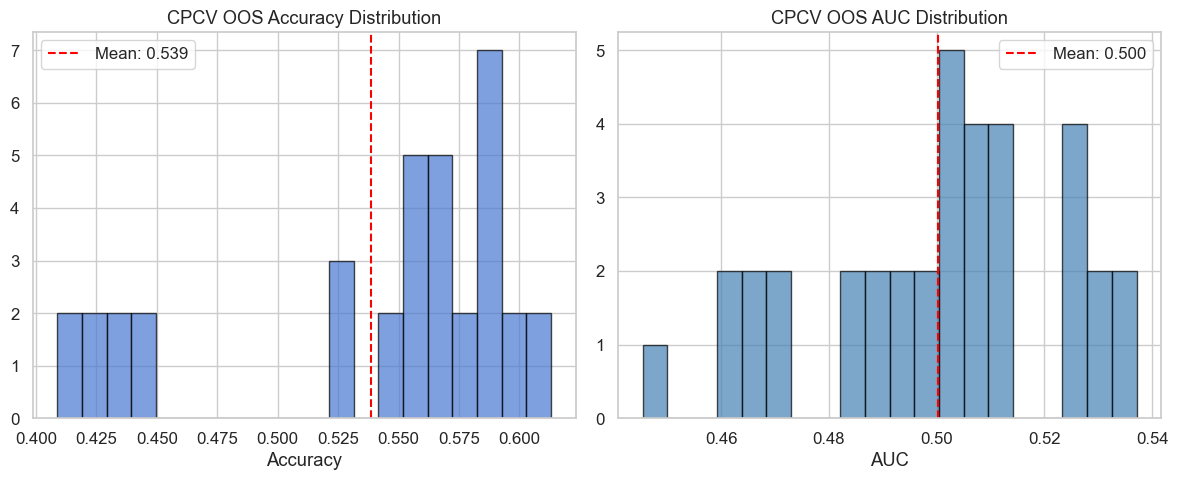
\includegraphics[width=0.95\linewidth]{figures/nb_cell48_out2.png}
\caption{Distribution of CPCV out-of-sample accuracy and AUC across 36 folds. Red dashed lines mark fold means (accuracy $\approx$0.539, AUC $\approx$0.500), matching Table E.2.}
\end{figure}

\subsection*{E.3 Test-Set Classification Metrics}
\begin{table}[h]
\centering
\begin{tabular}{lcccc}
\toprule
\textbf{Model} & \textbf{Accuracy} & \textbf{AUC} & \textbf{Precision (+)} & \textbf{Recall (+)} \\
\midrule
Stratified Dummy & 51.6\% & 0.500 & 0.531 & 0.516 \\
XGBoost (primary) & 53.1\% & 0.502 & 0.550 & 0.620 \\
\bottomrule
\end{tabular}
\caption{Test-set classification: XGBoost vs.\ stratified dummy baseline. The model's value lies not in ranking power (AUC $\approx$ 0.50) but in calibrated probabilities that enable effective bet sizing.}
\end{table}

\subsection*{E.4 Probability Calibration}
\begin{table}[h]
\centering
\begin{tabular}{lc}
\toprule
\textbf{Metric} & \textbf{Value} \\
\midrule
Brier score (model) & 0.247 \\
No-skill climatology Brier (predict base rate) & 0.249 \\
Expected Calibration Error (10-bin) & 0.018 \\
\bottomrule
\end{tabular}
\caption{Calibration diagnostics. The model improves slightly versus a no-skill climatology baseline on Brier score, while low ECE indicates small average probability-frequency gaps. A reliability diagram is reported in the notebook calibration artifact and should be interpreted jointly with these scalar metrics.}
\end{table}

\subsection*{E.5 Label Balance by Split}
\begin{table}[h]
\centering
\begin{tabular}{lcc}
\toprule
\textbf{Metric} & \textbf{Train} & \textbf{Test} \\
\midrule
Observations & 59,533 & 4,759 \\
Positive (TP hit) \% & 61.8\% & 53.1\% \\
Negative (SL hit / timeout) \% & 38.2\% & 46.9\% \\
\bottomrule
\end{tabular}
\caption{The shift from 61.8\% to 53.1\% positive labels confirms a genuine regime change in 2025, explaining the Sharpe degradation from validation (1.06) to test (0.41).}
\end{table}

\clearpage
\section{Bet Sizing Grid Search}
Supports: Sections 2.4, 3.2

\subsection*{F.1 Top Grid Search Configurations (Validation Period)}
\begin{table}[h]
\centering
\begin{tabular}{clclccc}
\toprule
\textbf{Rank} & \textbf{Method} & \textbf{Min Prob} & \textbf{Long Leg} & \textbf{Max Cap} & \textbf{Sharpe} & \textbf{Return} \\
\midrule
1 & half\_kelly & 0.49 & top\_decile & 5\% & 1.064 & 55.0\% \\
2 & half\_kelly & 0.49 & top\_decile & 10\% & 1.064 & 55.0\% \\
3 & half\_kelly & 0.51 & top\_decile & 5\% & 1.037 & 53.8\% \\
4 & half\_kelly & 0.51 & top\_decile & 10\% & 1.037 & 53.8\% \\
5 & meta\_prob & 0.51 & top\_vigintile & 10\% & 0.998 & 85.8\% \\
\bottomrule
\end{tabular}
\caption{Top 5 configurations by Sharpe on validation. Row 1 was selected for the final test. The top two configurations are identical at the 5\% vs.\ 10\% cap, suggesting robust performance insensitive to the cap choice.}
\end{table}

\subsection*{F.2 Grid Search Robustness}
Of the 48 configurations tested, 42 produced positive Sharpe ratios on the validation period. The top 10 configurations all used half-Kelly sizing with top-decile selection, varying only in meta-probability threshold (0.49--0.53) and cap level. This consistency across the grid provides evidence that the selected configuration is not an outlier driven by overfitting to one parameter combination.

\section{Risk Neutralization}
\subsection*{G.1 Neutralization Validation Report}
\begin{table}[h]
\centering
\begin{tabular}{lcccc}
\toprule
\textbf{Factor} & \textbf{Slope} & \textbf{P-Value} & \textbf{R-Squared} & \textbf{Neutralized} \\
\midrule
Sector (GICS dummies) & 0.000 & 1.000 & 0.000 & Yes \\
Size (log market cap) & 0.000 & 1.000 & 0.000 & Yes \\
Beta (vol\_20d proxy) & 0.083 & 0.000 & 0.004 & No \\
\bottomrule
\end{tabular}
\caption{Sector and size are fully neutralized. Beta neutralization was attempted but a residual loading persists ($R^2 = 0.004$), representing a small and economically negligible market-beta tilt.}
\end{table}

\section{Backtest \& Portfolio Performance}
Supports: Sections 1, 3.3, 4

\subsection*{H.1 Full Performance Metrics (Net of Costs)}
\begin{table}[h]
\centering
\begin{tabular}{lr}
\toprule
\textbf{Metric} & \textbf{Value} \\
\midrule
Total Return & 7.40\% \\
Annualized Return & 6.71\% \\
Annualized Volatility & 16.50\% \\
Sharpe Ratio & 0.41 \\
Sortino Ratio & 0.54 \\
Maximum Drawdown & $-$18.11\% \\
Calmar Ratio & 0.37 \\
Daily Hit Rate & 51.62\% \\
Monthly Positive \% & 57.14\% \\
Trading Days & 277 \\
Rebalance Dates & 8 (monthly) \\
Avg.\ Long Positions per Rebalance & $\approx$60 (top decile) \\
\bottomrule
\end{tabular}
\caption{Complete out-of-sample performance, net of 7.5\,bps/side costs, t+1 staggered execution.}
\end{table}

\subsection*{H.2 Regime-Decomposed Performance}
Market regimes were classified using trailing 126-day cumulative S\&P 500 returns, binned into bull ($>$10\%), sideways ($-$10\% to 10\%), and bear ($<-$10\%) categories. No bear regime occurred during the January--October 2025 test window. Four trading days at regime boundaries are excluded from the decomposition.

\begin{table}[h]
\centering
\begin{tabular}{lcc}
\toprule
\textbf{Metric} & \textbf{Sideways (167 days)} & \textbf{Bull (106 days)} \\
\midrule
Total Return & 7.51\% & 10.60\% \\
Annualized Return & 11.55\% & 27.07\% \\
Annualized Volatility & 17.97\% & 10.51\% \\
Sharpe Ratio & 0.64 & 2.58 \\
Sortino Ratio & 0.98 & 4.41 \\
Maximum Drawdown & $-$10.03\% & $-$3.90\% \\
\bottomrule
\end{tabular}
\caption{Regime-decomposed performance. The strategy captures strong alpha in trending markets and remains profitable in sideways conditions.}
\end{table}

\clearpage
\section{SHAP Explainability \& Model Transparency}
Supports: Sections 4.2, 4.4

SHAP (SHapley Additive exPlanations) analysis reveals that the model's predictions are driven primarily by \textbf{growth} (revenue\_growth\_yoy, net\_income\_growth\_yoy), \textbf{value} (earnings\_yield), and \textbf{volatility} (vol\_60d, gk\_vol\_20d, mdd\_126d) features. Momentum features contribute but are not the dominant driver. This is consistent with the model learning to identify quality/growth stocks with controlled volatility profiles.

\begin{figure}[h]
\centering
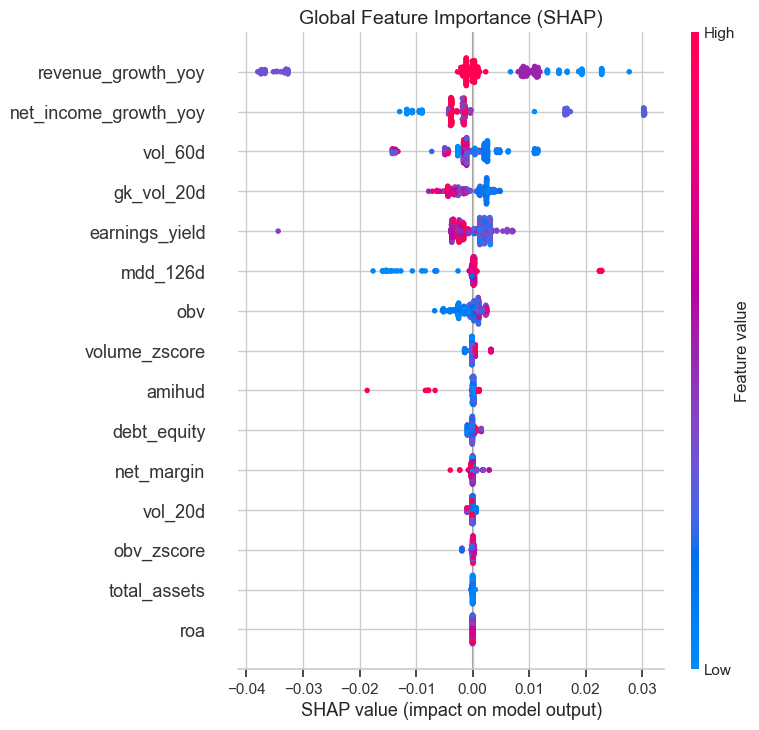
\includegraphics[width=0.72\linewidth]{figures/nb_cell47_out1.png}
\caption{Global SHAP summary plot. The highest-impact features are led by revenue growth, net income growth, earnings yield, and volatility variables, consistent with the narrative in this section.}
\end{figure}

\begin{figure}[h]
\centering
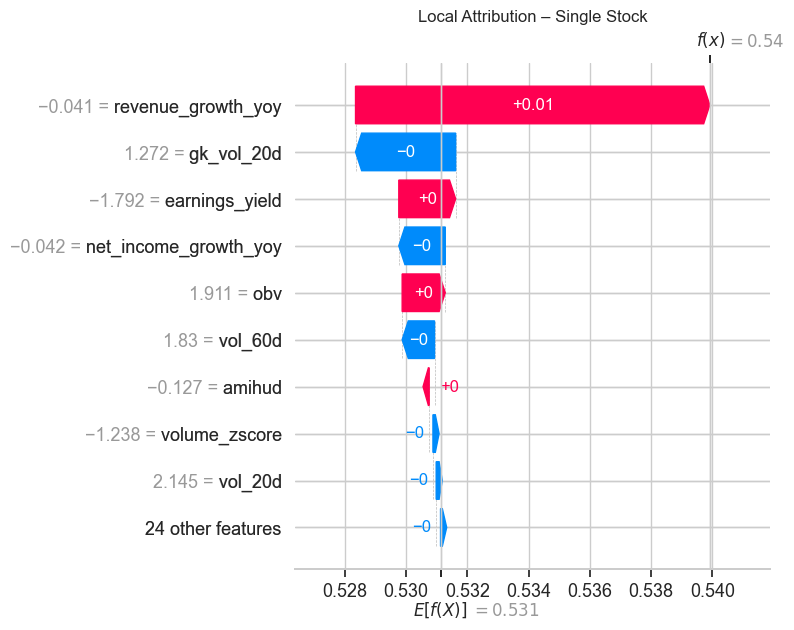
\includegraphics[width=0.72\linewidth]{figures/nb_cell47_out2.png}
\caption{Local SHAP decomposition for a representative single-stock prediction. The plot shows additive feature contributions from the baseline score to the final model output.}
\end{figure}

\subsection*{I.1 PM Decision Ledger (Sample Recommendations)}
\begin{table}[h]
\centering
\begin{tabular}{clllc}
\toprule
\textbf{Rank} & \textbf{Ticker} & \textbf{Sector} & \textbf{Direction} & \textbf{Meta Conviction} \\
\midrule
1 & DUK & Utilities & Long & 0.720 \\
2 & CMS & Utilities & Long & 0.719 \\
3 & NI & Utilities & Long & 0.719 \\
4 & LNT & Utilities & Long & 0.719 \\
5 & EVRG & Utilities & Long & 0.719 \\
\bottomrule
\end{tabular}
\caption{Top-ranked recommendations from the most recent rebalance. Utilities concentration is mitigated by the 30\% sector cap in the portfolio construction layer.}
\end{table}

\section{Observation-Level Return Diagnostics}
\subsection*{J.1 Scored vs. Allocated Observation Statistics}
\begin{table}[h]
\centering
\begin{tabular}{lc}
\toprule
\textbf{Metric} & \textbf{Value} \\
\midrule
Total test observations scored & 4,759 \\
Observations with non-zero weight & 2,310 (48.5\%) \\
Winning scored observations & 2,391 (50.2\%) \\
Losing scored observations & 2,368 (49.8\%) \\
Average return (all scored) & +1.32\% \\
Average winner & \textbf{+10.45\%} \\
Average loser & \textbf{$-$7.90\%} \\
Profit factor & \textbf{1.34} \\
Best single return & +242.84\% (SNDK) \\
Worst single return & $-$59.55\% (SMCI) \\
Unique tickers scored & 597 \\
\bottomrule
\end{tabular}
\caption{Observation-level return diagnostics. Counts above separate the full scored universe from the non-zero-weight allocated subset to avoid trade-count ambiguity.}
\end{table}

\section{Data Integrity Audit}
Supports: Sections 1, 3

\subsection*{K.1 Data Leakage Audit Summary}
\begin{table}[h]
\centering
\small
\begin{tabular}{cp{3.5cm}p{3.5cm}p{3.5cm}}
\toprule
\textbf{\#} & \textbf{Issue} & \textbf{Resolution} & \textbf{Impact} \\
\midrule
1 & Early stopping used test data & Carved internal val from train & Prevents model selection leak \\
2 & Backtest started at $t$ & Shifted to $t+1$ execution & No same-day return capture \\
3 & Neutralization used full window & Per-date cross-sectional only & No future exposure info \\
4 & No 3-way split for sizing & Added validation period & Params unexposed to test \\
\bottomrule
\end{tabular}
\normalsize
\caption{Four leakage fixes applied during development.}
\end{table}

\subsection*{K.2 Key Safeguards Implemented}
\begin{table}[h]
\centering
\begin{tabular}{p{0.25\linewidth} p{0.7\linewidth}}
\toprule
\textbf{Safeguard} & \textbf{Description} \\
\midrule
PIT fundamentals & All filings anchored to SEC acceptance date, not fiscal period end \\
Survivorship-free & 801 tickers including $\sim$298 historically removed companies \\
CPCV validation & 36 purged folds with 5-day embargo prevent temporal leakage \\
Three-way split & Train / Validation / Test ensures bet sizing is not optimized on test \\
t+1 execution & Signals at close of $t$, execution begins at $t+1$ \\
Transaction costs & 7.5\,bps/side applied to all reported metrics \\
Risk neutralization & Sector and size fully orthogonalized; residual beta tilt is negligible ($R^2 = 0.004$) \\
FRED vintage & Macro layer uses current-vintage FRED; strict PIT vintage reconstruction would require ALFRED/release-aware handling \\
\bottomrule
\end{tabular}
\caption{Complete list of pipeline safeguards.}
\end{table}

\end{document}